\chapter{Anforderungen}
\label{chap:Anforderungen}
Dieses Kapitel beschreibt die Anforderungen der beiden Seiten an den Elektrolyseur. Auf der einen fordert der Versorgungsnetzbetreiber u.a. die Einhaltung der \gls{VDE} Richtlinien für den Anschluss an das Stromnetz. Die andere Seite wird vom Hersteller der Elektrolyseur Stacks definiert, wozu es nach heutigem Stand keine Standards gibt.
\section {Stromnetz} \label{sec:AnfStromnetz}
In Deutschland sind die Vorgaben für den Anschluss von Anlagen an das Stromnetz durch den \gls{VDE} definiert. Je nach Anschlussleistung, Standort und Betriebsverhalten, wird eine unterschiedliche Netzspannungsklasse gewählt, welche geringfügig abweichende Anschlussrichtlinien besitzt. Aufgrund der Skalierbarkeit zu höheren Leistungsklassen und der erwartbar steigenden Anforderungen, wird sich für die Anforderungen der Hochspannung entschieden. Diese hat die Bezeichnung VDE-AR-N 4120 "Technische Regeln für den Anschluss von Kundenanlagen an das Hochspannungsnetz und deren Betrieb (TAR Hochspannung)" \cite{VDEARN4120}.
Hierzu zählt unter anderem die Anforderung an die Phasenverschiebung, bei Wirkleistungsbezug darf eine maximale Verschiebung von $cos(\phi)=0,95$ was einem Winkel von etwa 18 Grad entspricht auftreten vgl. Abb. \ref{fig:tar4120pq}. Jedoch kann der Netzbetreiber mit dem Anlagenbetreiber gesonderte Vereinbarungen treffen, dies ermöglicht es Netzdienstleistungen anzubieten. Dies führt zur Anforderung an die Topologie eine Phasenverschiebung von mindestens 18 Grad zu ermöglichen.\\
\begin{figure}[H]
	\centering
	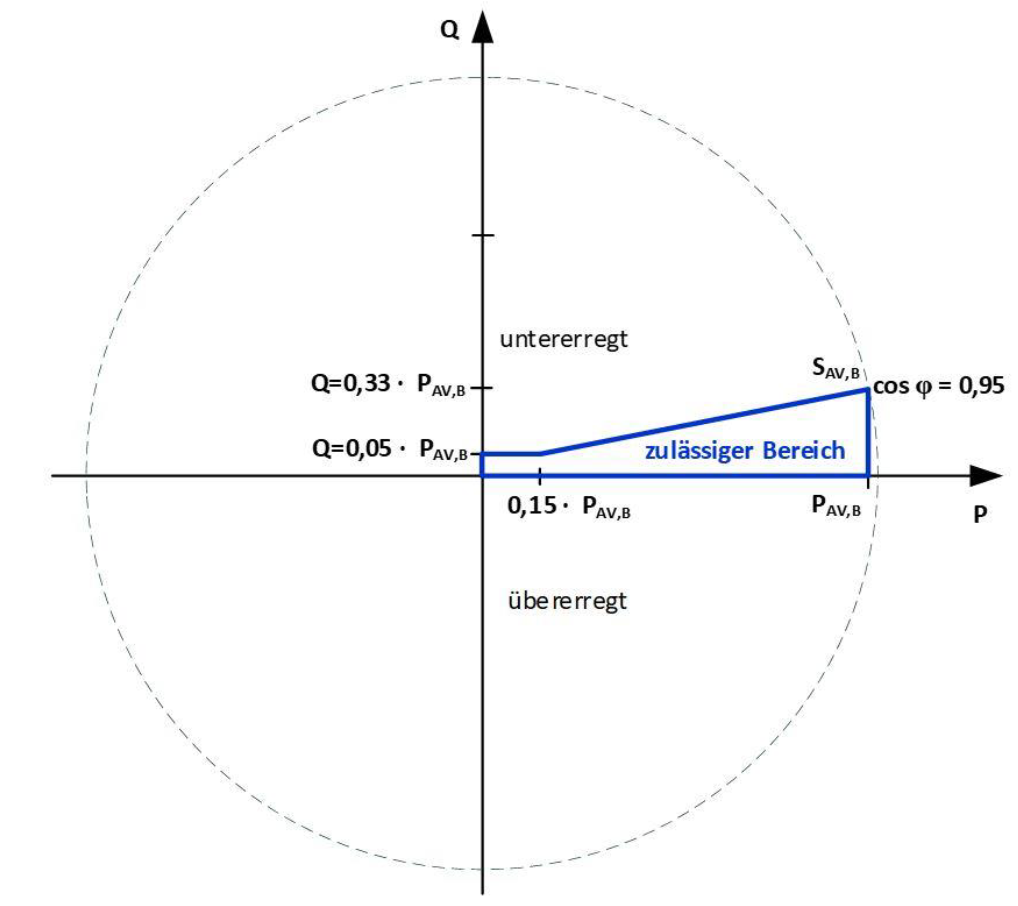
\includegraphics[width=0.6\linewidth]{content/Grafiken/TAR4120_PQ}
	\caption[Zulässiger Bereich des Verschiebungsfaktors cos $\phi$ bei Wirkleistungsbezug]{VDE TAR4120: Zulässiger Bereich des Verschiebungsfaktors \cite{VDEARN4120}}
	\label{fig:tar4120pq}
\end{figure}
Des weiteren sind zeitlich begrenzte Frequenz und Spannungsänderung die auftreten können definiert als quasistationärer Betrieb. Die Netzspannung kann im Bereich von +/- 15 Prozent Schwanken, sowie die Frequenz von 50 Hertz zwischen 47,5 und 51,5 variieren vgl. Abb \ref{fig:vde4120-Anforderungen} (a). Innerhalb dieses Bandes muss die Anlage im regulären Betrieb bleiben. Dabei wird ein Gradient von  <5 \%  im Spannungsband sowie <0,5 \% pro Minute im Frequenzband vorausgesetzt. \\
Im Fehlerfall durch Blitzeinschlag oder Kurzschluss, muss die Anlage kurzzeitig deutlich stärkere Spannungsschwankungen mit machen. Diese Anforderung wird als \gls{FRT} bezeichnet und kann für bis zu 100 Millisekunden die Spannung um 25 Prozent erhöhen vgl. Abb. \ref{fig:vde4120-Anforderungen} (b). Aufgrund eines Kurzschluss kann die Spannung auf 15 Prozent der eigentlichen Netzspannung abfallen. Dies stellt für Verbraucheranlagen eine große Herausforderung dar, da die zu betreibenden Systeme meist eine minimal Spannung benötigen.

\begin{figure}[H]
\centering
\subfloat[][]{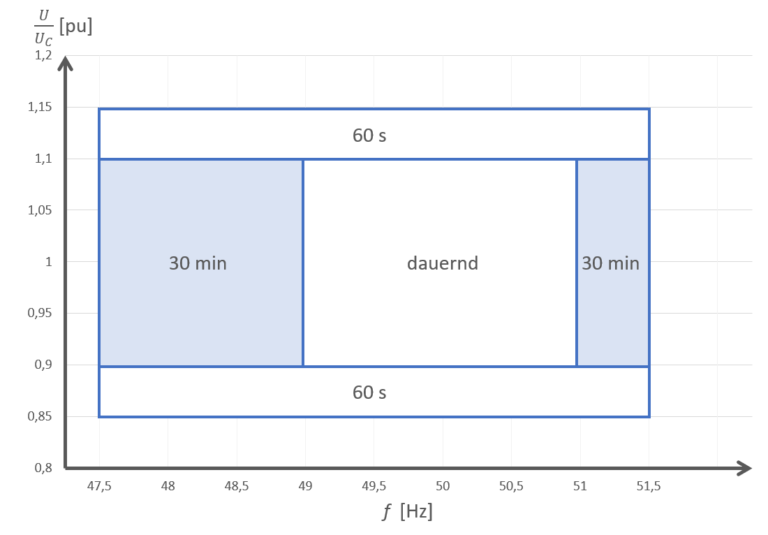
\includegraphics[width=0.7\linewidth]{content/Grafiken/VDE4120-quasistationarerbetrieb}}%
%\caption[Mindestanforderungen an den quasistationären Betrieb von Erzeugungsanlagen \cite{VDEARN4120]{Quasistationärer Betrieb}}

\qquad
\subfloat[][]{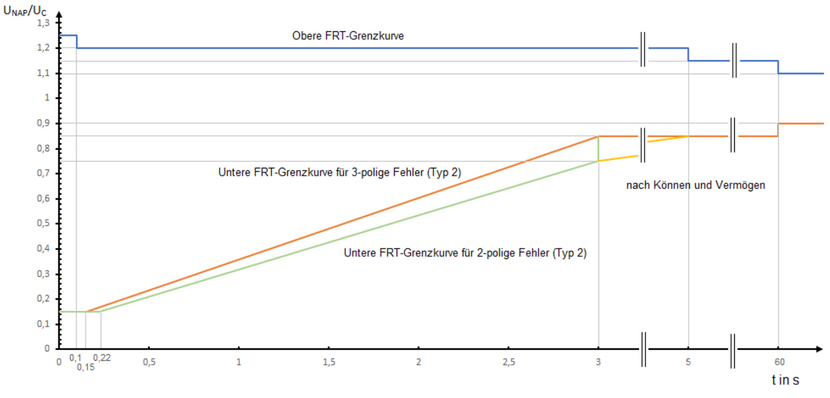
\includegraphics[width=0.7\linewidth]{content/Grafiken/Grenzkurve}}%

\caption[quasistationären Betrieb (a) und \gls{FRT} (b)]{Mindestanforderungen an den quasistationären Betrieb (a) und \gls{FRT} (b)}
\label{fig:vde4120-Anforderungen}
\end{figure}




	\subsection{Systemdienstleistungen (SDL)}
	Generell ist die Bundesnetzagentur für die Regulierung und Kontrolle von jeglichen Dienstleistungen und Aktivitäten im deutschen Netz zuständig. Dazu gehört auch die Bereitstellung und Gewährleistung von Blindleistung, neben der Wirkleistung, diese soll effizient, transparent und Diskriminierungsfrei am Markt beschafft werden \cite{Bundesnetzagentur}. Dazu bieten sich zukünftig große Verbrauchsanlage wie Elektrolyseure neben Erzeugungsanlagen an und diese Dienstleistungen können die Wasserstofferzeugung wirtschaftlicher machen.\\
	 Die Systemdienstleistungen werden nach VDE-ARN 4141-1 in vier Kategorien unterteilt, diese sind Frequenz- und Spannungshaltung, Netzwiederaufbau und die Betriebsführung. Durch \gls{TAR} werden diese definiert und Anforderungen für Nachweise und Ausschreibungen von \gls{SDL} gestellt. Eine Übersicht über die technischen Mindestanforderungen an Erzeugungsanlagen in den verschiedenen Spannungsklassen ist in Abb. \ref{fig:vde-fnn-tar} dargestellt. Für Stromrichter basierte Elektrolyseanlagen stellen Frequenzschwankungen kaum eine Herausforderung, diese können über Regelungsvorgänge kompensiert und Netzstützung ,wie bei \gls{RoCoF} benötigt, bereitgestellt werden. Bei \gls{RoCoF} handelt es sich um schnelle Frequenzänderungen, wie bei einer Netzauftrennung oder Wiederverknüpfung. Primärregelleistung, statische Spannungshaltung und Dynamische Netzstützung können ebenfalls durch Regelungsverhalten implementiert werden, jedoch begrenzt durch die Dynamik und den Leistungsbezug des Elektrolyseurs. Netzrückwirkungen müssen ebenfalls betrachtet und können durch entsprechende Filter kompensiert werden. Die Schwarzstartfähigkeit gestaltet sich in dem Falle schwierig und kann nur durch Leistungsbegrenzung während des Wiederaufbaus unterstützt werden.
	\begin{figure}
		\centering
		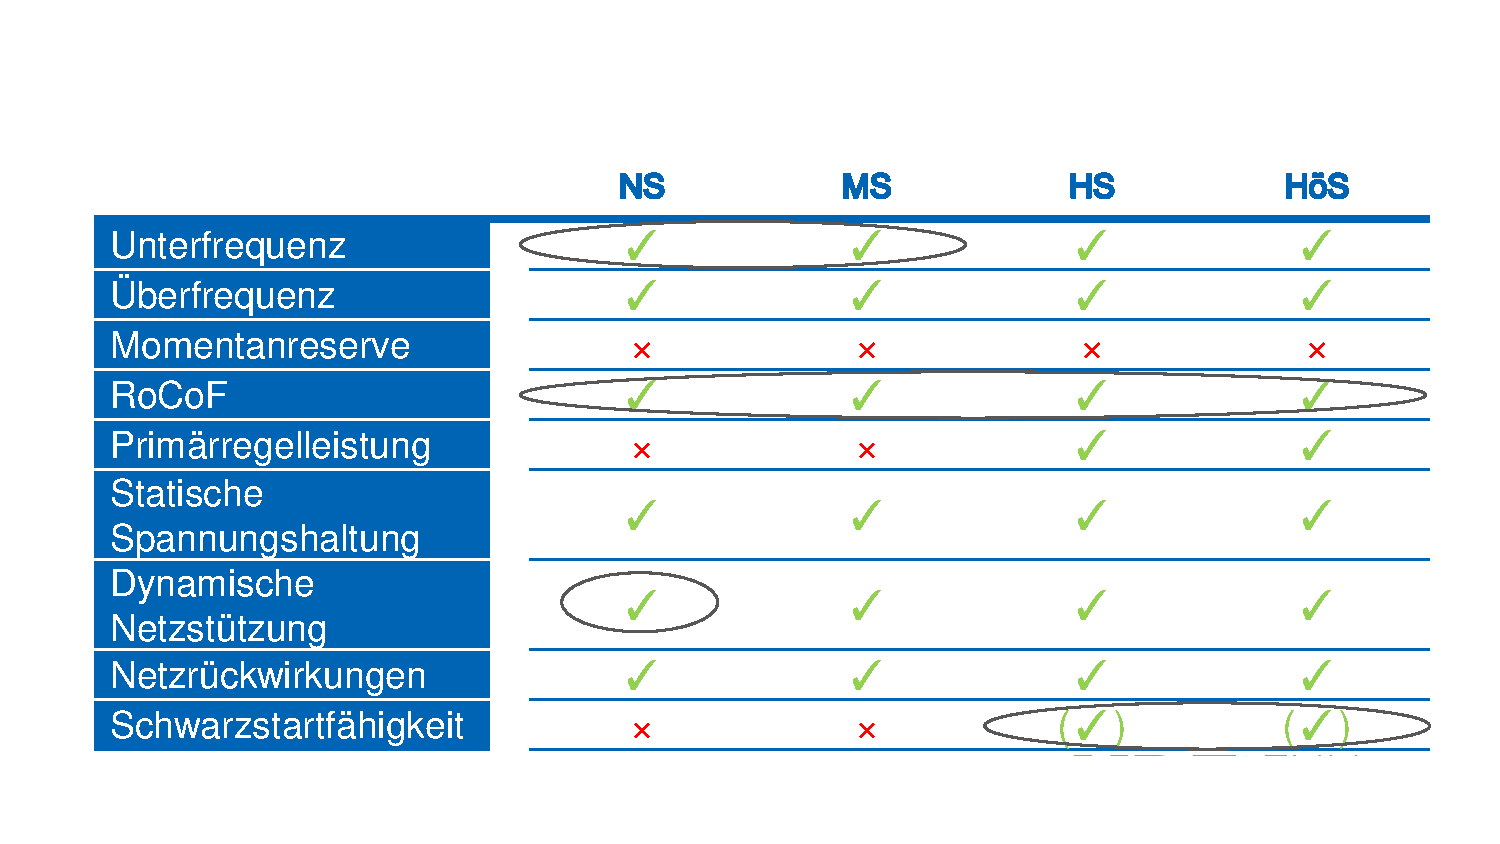
\includegraphics[width=0.9\linewidth]{content/Grafiken/VDE-FNN-TAR}
		\caption[Technischen Mindestanforderungen an Erzeugungsanlagen Stand 2019]{Technischen Mindestanforderungen an Erzeugungsanlagen Stand 2019 \cite{VDEFNN2019SDL}}
		\label{fig:vde-fnn-tar}
	\end{figure}
	
	
	
	
	\subsection{Fault-Ride-Through (FRT))}
	Aufgrund von Netzfehlern oder Blitzeinschlag, kann es zu kurzfristiger Erhöhung der Netzspannung kommen, dies wird als Überspannung bezeichnet. Aufgrund dieser Spannungserhöhung kann es zur Fehlfunktion bis hin zur Zerstörung von Anlagenteilen kommen. Um die Anlage innerhalb der Norm betreiben zu können, müssen Schutzmaßnahmen getroffen werden, um einen Ausfall der Anlage und Schutz der dahinter liegenden Komponenten zu Gewährleisten.  \\
	
	Wichtig hierbei ist es insbesondere bei Spannungseinbrüchen, dass der Wirkleistungsbezug nach dem Fehler wieder möglichst schnell auf das Niveau vor dem Fehler zurückkehrt, falls dieser Reduziert wurde. Dies wird von den vier in Deutschland zuständigen Übertragungsnetzbetreibern gefordert \cite{4UNB}.


\section{Elektrolyseur}
Zur Elektrolyse wird eine Gleichspannung benötigt welche aufgrund von Alterungsprozessen, innerhalb der Zellmembrane, mit der Zeit ansteigt \cite{HydrogenElectronicTopologies}. Außerdem wird zu Beginn der Elektrolyse eine niedrige Spannung benötigt um den Prozess zu starten. Daher wird ein Bandbreite von 0 bis einigen 100 Volt benötigt. Um die gewünschte Leistung umsetzen zu können ist es für die Wirtschaftlichkeit relevant den Strom möglichst zu reduzieren, woraus eine höhere Spannung resultiert. Dies wird durch den modularen Zellaufbau unterstützt der eine Flexible Systemspannung ermöglicht. \\
Um die Effizienz und Lebensdauer des Elektrolyseurs nicht zu reduzieren, wird ein maximaler Stromrippel angegeben. Dieser liegt zwischen 5 und 10 Prozent bei Anlagen bis drei Megawatt, für größere Leistungen und zukünftige Anwendungen soll er kleiner als drei Prozent sein \cite{HydrogenRectifier}.


\section{Zusammenfassung}
Die Anforderungen an den Gleichrichter sind in Tabelle \ref{tab:AnfZsm} zusammengefasst, für die Implementierung werden die Zukünftigen Anforderungen als relevant betrachtet.\\
\begin{table}
\caption{Anforderungen an den Gleichrichter Aktuell und in Zukunft}

\begin{tabular}{c|c|c}
	
	& Aktuell & Zukünftig \\
	\hline
	Leistungsfaktor stationär & >0.95 & >0.99 \\
	\hline
	Leistungsfaktor als Systemdienstleistung & keine Angabe & +/- 30° \\
	\hline
	Ausgangsstromrippel & <5 \% & <2 \% \\
	\hline
	Ausgangsspannung & < 1000 V & < 1500 V \\
	
	
	\label{tab:AnfZsm}
\end{tabular}
\end{table}
\section{Bewertungskriterien}
Die Kriterien zur finalen Auswahl der Topologie setzen sich aus der Erfüllung der Anforderungen zusammen sowie der Bewertung der Hardware. Die Grundlegenden Anforderungen aus Seiten des Stromnetzes und Elektrolyseur wurden bereits in der Vorauswahl berücksichtigt und können nun im Detail anhand von \gls{THD} und Rippelgrößen betrachtet werden. Die Quantifizierung der Hardware wird zum einen anhand der Verlustleistung in den Halbleitern, welche indirekt auch den Kühlungsaufwand repliziert, zum anderen durch die Größe und den Aufwand für die Komponenten berücksichtigt.  